\documentclass{article}

\textwidth=6.5in
\textheight=8.5in
\voffset=-54pt
\oddsidemargin=0in
\evensidemargin=0in
\setlength{\parskip}{8pt}
\setlength{\parindent}{0pt}

\usepackage{amsmath, amssymb}
\usepackage{ifthen}

\usepackage[inline]{enumitem}
\setlist{topsep=0pt, parsep=8pt}

\usepackage[rgb,table]{xcolor}\convertcolorsUfalse
\usepackage{graphicx}

% change hyperref options
\PassOptionsToPackage{hyphens}{url}
\usepackage[bookmarks,colorlinks,linkcolor=black,citecolor=blue,pdfstartview=FitH,urlcolor=blue]{hyperref}
\hypersetup{pdfpagemode=UseNone}
\usepackage{bookmark}

\usepackage{graphicx}
\usepackage{multicol}
\usepackage{framed}
\usepackage{array}

\usepackage{icomma}

\usepackage{soul}
\usepackage[normalem]{ulem}

\usepackage{pgfplots}
\pgfplotsset{compat=1.18}  
\pgfplotscreateplotcyclelist{mycolor}{black, blue, red, green!70!black, magenta, purple, cyan, orange }  
\pgfplotsset{
  disabledatascaling,
  cycle list=tikzcolor, 
  axis lines=middle,
  every axis plot/.style={no marks, thick},
  every axis/.style={
    enlarge x limits=false,
    enlarge y limits=auto,
    xlabel style={at={(current axis.right of origin)},anchor=west},
    ylabel style={at={(current axis.above origin)},anchor=south},
    % extra x and y ticks for asymptotes
    extra x tick style={grid=major, grid style={dashed,black}},
    extra y tick style={grid=major, grid style={dashed,black}},
    /pgf/number format/1000 sep={},
  },    
  tick label style = {font=\footnotesize, fill=\currentbgcolor, inner sep=0pt},    
  xticklabel shift=1pt,    
  scaled ticks=false,
  scaled y ticks=false,
  unbounded coords=jump,
  samples=101,
  minor tick length=0,
  scatter/classes={
    open={mark=*,draw=black,fill=white, mark size=2, thin},
    closed={mark=*,draw=black,fill=black, mark size=2, thin}
  },
  width=3in,
}
\pgfplotsset{open/.style={only marks, mark=*, fill=white, thin, mark size=2}}
\pgfplotsset{closed/.style={only marks, mark=*, draw=black, fill=black,
    thin, mark size=2}}
\pgfplotsset{labeled/.style={nodes near coords, only marks, mark=*, draw=black, fill=black, thin, mark size=2, point meta=explicit symbolic}}

\usepackage{tikz}
\usetikzlibrary{
  matrix,%
  % enables the snake paths
  decorations.pathmorphing,%
  % enables bigger arrows
  decorations.markings,%
  decorations.pathreplacing,%
  decorations.text,%
  calc,%
  patterns,%
  shapes.geometric,%
  arrows,
  decorations.shapes,
  positioning,
  plotmarks,
  intersections
}
\tikzset{>=latex} % sets default arrow type in tikz
\tikzset{font=\normalsize}
\tikzset{mark size=1.5pt, mark options=thin}
\tikzset{pin distance=4pt,
  every pin edge/.style={<-, thin, shorten <= -2pt}}

\interfootnotelinepenalty=10000
\renewcommand{\thefootnote}{(\arabic{footnote})}

\usepackage{multirow, bigdelim}

% change to \usepackage[sols]{handout} to see solutions
\usepackage[sols]{handout}
\renewcommand{\workshopnote}{CA Notes.}    

\newcommand\iscurrentenumi[1]{%
  \ifthenelse{\equal{#1}{\theenumi}}{}{#1}}
\setenumerate[1]{ref=\#\arabic*}
\setenumerate[2]{ref=\protect\iscurrentenumi{\theenumi}(\alph*)}
\newcommand\enumiiprefix[2]{%
  \ifthenelse{{\equal{#1}{\theenumi}}\AND{\equal{#2}{(\alph{enumii})}}}{}{}%
  \ifthenelse{{\equal{#1}{\theenumi}}\AND{\NOT{\equal{#2}{(\alph{enumii})}}}}{#2}{}%
  \ifthenelse{\equal{#1}{\theenumi}}{}{#1#2}%
}
\setenumerate[3]{ref=\protect\enumiiprefix{\theenumi}{(\alph{enumii})}\roman*}

\makeatletter

% underline links               
\let\@href=\href
\renewcommand{\href}[2]{\@href{#1}{\ul{#2}}}
\usetikzlibrary{backgrounds}
\tikzset{%
  fancy quotes/.style={
    text width=\fq@width pt,
    align=justify,
    inner sep=1em,
    anchor=north west,
    minimum width=\linewidth,
  },
  fancy quotes width/.initial={.8\linewidth},
  fancy quotes marks/.style={
    scale=8,
    text=white,
    inner sep=0pt,
  },
  fancy quotes opening/.style={
    fancy quotes marks,
  },
  fancy quotes closing/.style={
    fancy quotes marks,
  },
  fancy quotes background/.style={
    show background rectangle,
    inner frame xsep=0pt,
    background rectangle/.style={
      fill=blue!10!white,
      rounded corners,
    },
  }
}
\newcommand{\fancyquoteattrib}{}
\newcommand*\quotefont{\fontfamily{LinuxLibertineT-LF}} % selects Libertine 
\newenvironment{fancyquote}[1][]{%
  \noindent
  \tikzpicture[fancy quotes background]
  \node[fancy quotes opening,anchor=north west] (fq@ul) at (0,0) {\quotefont\selectfont``};
  \tikz@scan@one@point\pgfutil@firstofone(fq@ul.east)
  \pgfmathsetmacro{\fq@width}{\linewidth - 2*\pgf@x}
  \node[fancy quotes,font=\normalsize,#1] (fq@txt) at (fq@ul.north west) \bgroup}
{\egroup;
  \node[overlay,fancy quotes closing,anchor=east] at (fq@txt.south east) {\quotefont\selectfont''};
  \draw (fq@txt.south east) node[left, xshift=-32pt, yshift=-4pt] {--- \fancyquoteattrib}; 
  \endtikzpicture}

\makeatother

\definecolor{purple}{rgb}{0.5,0,1.0}

\definecolor{skyblue}{rgb}{0, 0.5, 1}

\newcommand{\doedfinity}[2][\newpage]{
  \begin{problem}[#1]
    Do the Edfinity assignment ``Problem Set #2''.

    We encourage you to write down any scratch work here, as well as
    things you want your future self to remember. Nothing you write
    here will be graded; it's just for you!
  \end{problem}
}

\newcommand{\psreflection}[2][]{

  \ifthenelse{\not\equal{#1}{nocite}}{
    \begin{enumerate}[resume]
    \item
      \begin{problem}[1in]
        Please cite any help you got on this problem set:
        \begin{itemize}[nosep]
        \item If you worked with other students, please list their names here.
        \item If you used resources other than those on our Canvas site, please list them here.
        \end{itemize}
      \end{problem}

    \end{enumerate}
  }

  \probonly{%
    #2

    \newpage

    \emph{Reflection space.} It's a good habit to take a few minutes at the end of each pset to reflect on what you learned and jot down notes to your future self. Here are a few reflection questions to get you started. Nothing you write here will be graded; it's just for you!
    \begin{itemize}
    \item Take a few minutes to look back at the problems. How could you explain to someone else how to do each problem? What was your strategy, and how did you know to use that strategy? If there are problems where you don't feel able to answer this, write down which ones they are. Come back to them in a few days when we post the homework solutions!

      \vspace{1.5in}

    \item Take a look back at the learning objectives on today's worksheet; how are you feeling about each one? If there are ones you know you need more practice with, write those down here.

      \vspace{1.5in}

    \item What did you find most challenging about this material? Do you have any lingering questions about it? If so, write them down here so you don't forget them. At some point, stop by office hours or MQC to ask!

      \vfill
    \end{itemize}      
  }
}

\usepackage{fancyhdr}
\lhead{\textcolor{white}{This content is protected and may not be shared, uploaded, or distributed.}}
\rhead{}
\rfoot{\vspace*{\fill}\footnotesize\textcopyright{} \emph{Harvard Math Ma}}
\renewcommand{\headrulewidth}{0pt}
\pagestyle{fancy}
\begin{document}

\begin{center}
  \large\textsc{Problem Set 2 - A Library of Basic Functions and Properties}
\end{center}

\begin{grading}
  One goal of Math M is to help students develop their ability to communicate mathematical reasoning. So, give students feedback if their work or explanations are hard to follow. You don't have to be super specific; it's enough to say something like ``This is hard to follow; please stop by MQC or office hours to talk about communicating your reasoning''. 
\end{grading}

\begin{problemonly}
  \begin{tcolorbox}[colframe=skyblue, colback=white, 
    sharp corners, size=fbox, parbox=false, boxrule=0.5mm]
    {\large\textbf{\textsf{Homework Tips!}}}

    Homework is an essential part of your learning in Math M. Here are a few tips to help you get the most out of your homework assignments.    

    \textbf{\textsf{Start early!}}

    Start your assignment as soon as possible, even if you can only spend 15 minutes reading the problems. The assignments are your chance to think hard about the material and uncover your own misunderstandings; this can't happen properly if you don't give yourself time.

    \textbf{\textsf{Try each problem \emph{before} you talk with anyone else.}} \renewcommand{\fancyquoteattrib}{\href{https://www-degruyter-com.ezp-prod1.hul.harvard.edu/document/doi/10.4159/9780674419377/html}{\emph{Make It Stick: The Science of Successful Learning}}}

    \begin{fancyquote}
      Trying to come up with an answer rather than having it presented to you\ldots leads to better learning and longer retention of the correct answer or solution, even when your attempted response is wrong.
    \end{fancyquote}

    If you get stuck on a problem (and you should---the problems are intentionally challenging!), try to diagnose exactly why you're stuck so that you can effectively ask a classmate, CA, or TF for help.

    \textbf{\textsf{Discuss with your classmates}}

    Talk with your classmates about your ideas, and try to describe your strategies out loud. Ask each other lots of questions, and draw each other pictures to help explain. However, you should \textbf{not} look at other students' complete solutions. Please make sure you understand the collaboration policy in the \href{https://people.math.harvard.edu/~jjchen/mathma/docs/handouts/syllabus.html}{syllabus}.

    Even if you didn't need help doing the assignment, spend some time in office hours, MQC, or elsewhere to check your answers with classmates and talk over your solutions. There are lots of ways to solve many of the problems, and you'll get a lot out of explaining your thinking and listening to someone else's strategies. \renewcommand{\fancyquoteattrib}{\href{http://ideas.time.com/2011/11/30/the-protege-effect/}{Annie Murphy Paul}, a journalist who writes about the science of learning}

    \begin{fancyquote}
      For thousands of years, people have known that the best way to understand a concept is to explain it to someone else.
    \end{fancyquote}
  \end{tcolorbox}
\end{problemonly}

\begin{problemonly}
  \emph{Note:} On this problem set, you'll need to do some factoring; here's a \href{https://www.khanacademy.org/math/algebra/x2f8bb11595b61c86:quadratics-multiplying-factoring/x2f8bb11595b61c86:factor-quadratics-intro/v/factoring-simple-quadratic-expression}{refresher} on that.
\end{problemonly}

\begin{enumerate}
\item 

  \begin{grading}
    Nothing to turn in.
  \end{grading}

  As you saw in the tips, we encourage you to discuss the material and problem sets with others. In the next week or so, please either talk with someone at the Math Question Center (MQC) or office hours, or get together with at least one other student outside of class. We'll ask you to write a little about your experience on Problem Set 6 (due Wednesday 9/18) and to share in class, so that you can hear from your peers about what different resources are like.

  (You don't need to turn in anything for this problem right now.)

  \pspace{\newpage}

\item  \note{
    \begin{itemize}[nosep]
    \item Algebra: simplifying rational expressions
    \item Match the 7 basic functions with their graphs
    \item Some functions are neither even nor odd.
    \item Find the domain of a couple of functions. 
    \end{itemize}
  }

  \doedfinity{2}

\item % based on 2.1.6

  In each part, you're given a list of characteristics. Sketch a graph of a function that's continuous on $(-\infty, \infty)$ and has \uline{all} of the characteristics listed. Please label any important values on your axes; no explanation is necessary.

  \begin{enumerate}

  \item

    \begin{grading}
      1.5 points: 0.5 for each requirement (being negative, being increasing, being concave down)
    \end{grading}

    \begin{problem}[\vfill]
      On $(-\infty, \infty)$, $f$ is negative, increasing, and concave down. 
    \end{problem}

    \begin{solution}  
      \begin{center} 
        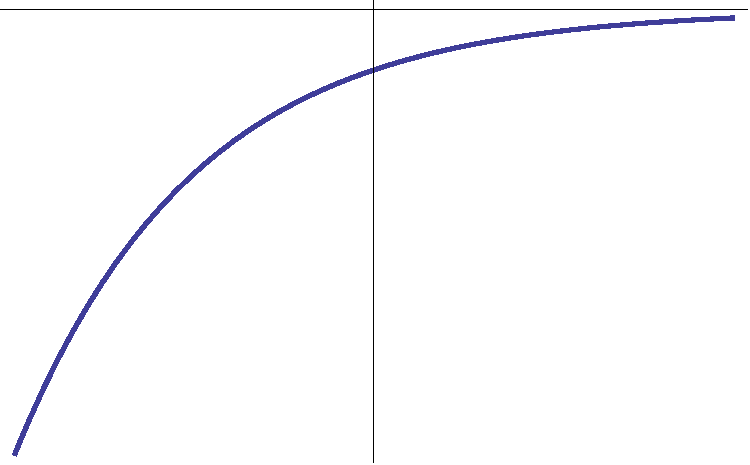
\includegraphics[width=2in]{images/negincccd.pdf}      
      \end{center} 
    \end{solution}

  \item

    \begin{grading}
      1.5 points: 0.5 for each requirement

      This graph just needs to be above $y = 5$; it doesn't have to
      have $y = 5$ as a horizontal asymptote. If they have a horizontal asymptote but haven't labeled 5 on the vertical axis, deduct 0.25. 
    \end{grading}

    \begin{problem}[\vfill]
      On $(-\infty, \infty)$, $f$ is decreasing and concave up and has lower bound 5.
    \end{problem}

    \begin{solution}        
      \begin{center} 
        \begin{tikzpicture}
          \begin{axis}[ymin=0, ytick={5}, xtick=\empty]
            \addplot+[domain=-3:3] {0.5^x + 5.5};
            \addplot+[dashed, domain=-3:3] {5};
          \end{axis}
        \end{tikzpicture}
      \end{center} 
    \end{solution}

  \item

    \begin{grading}
      1 point: 0.5 for each requirement

      We haven't specified the concavity their graph should have, so
      there are a lot of possibilities here. 
    \end{grading}

    \begin{problem}[\vfill]
      On $(-\infty, \infty)$, $f$ is increasing without bound. Also, $f$ has $x$-intercept 3. 
    \end{problem}

    \begin{solution}
    Here are some possible graphs.
    
      \begin{center}
      \begin{tabular}{c c c c c}
      
        \begin{tikzpicture}
          \begin{axis}[width=2in, ytick = \empty, xtick = {3}]
            \addplot[domain=-1:6]{x-3};
          \end{axis}
        \end{tikzpicture} &&
        
        \begin{tikzpicture}
          \begin{axis}[width=2in, ytick = \empty, xtick = {3}]
            \addplot[domain=-1:6]{(x-3)^3};
          \end{axis}
        \end{tikzpicture} &&
        
        \begin{tikzpicture}
          \begin{axis}[width=2in, ytick = \empty, xtick = {3}]
            \addplot[domain=-1:6]{e^x - e^3};
          \end{axis}
        \end{tikzpicture} 
        
      \end{tabular}
      \end{center}
      
    \end{solution}

  \item

    \begin{grading}
      3 points: 1 for each piece

      If their graph has the right behavior but they haven't labeled 2, 10 on the horizontal axis, deduct 0.25. 
    \end{grading}

    \begin{problem}[\vfill\newpage]
      $f$ is increasing and concave up on $(-\infty, 2)$, increasing and concave down on $(2, 10)$, and decreasing and concave down on $(10, \infty)$.
    \end{problem}

    \begin{solution}
      \begin{center}
          \begin{tikzpicture}
              \begin{axis}[xmin=-5.25, xmax=15.25, xtick=\empty, ytick=\empty, extra x ticks={2,10}]
                  \addplot[domain=-5.25:2]{4*rad(atan(x-2))+10};
                  \addplot[domain=2:15.25]{(-1/4)*(x-2)^2 + 4*x + 2};
              \end{axis}
          \end{tikzpicture}
      \end{center}
    \end{solution}

  \end{enumerate}

\item 

  Here are four functions:

  \[ f(x) = \frac{x}{x^2 + 1} \qquad g(x) = \frac{x^2}{x + 1} \qquad h(x) =
    \frac{4 x^2 - 1}{x^3} \qquad j(x) = \frac{x^2 - 1}{x^4 + 1} \]

  \begin{enumerate}
  \item \label{even-odd-functions} 

    \begin{grading}
      4 points: 1 point per function (if they correctly say whether a function is even, odd, or neither but have no justification or completely incorrect justification, give 0.25)
    \end{grading}

    \begin{problem}[\vfill]
      Algebraically determine whether each function is even, odd, or
      neither. Show your work.
    \end{problem}

    \begin{solution} 
    
      $f(-x) = \dfrac{-x}{(-x)^2 + 1} = - \dfrac{x}{x^2 + 1} = - f(x)$, so $f$ is odd.

      $g(-x) = \dfrac{(-x)^2}{-x + 1} = \dfrac{x^2}{-x + 1}$, which is not $g(x)$ or $-g(x)$. So, $g$ is neither even nor odd.

      $\displaystyle h(-x)= \frac{4(-x)^2-1}{(-x)^3} = \frac{4x^2-1}{-x^3} = -h(x)$, so $h$ is odd.

      $\displaystyle j(-x) = \frac{(-x)^2-1}{(-x)^4+1}= \frac{x^2-1}{x^4+1} = j(x)$, so $j$ is even.
    \end{solution} 

  \item

    \begin{grading}
      4 points, 1 per function: 0.25 for the right graph, 0.75 for a correct explanation

      Of course, they may have a different explanation from the one in the solution.
    \end{grading}

    \begin{problem}
      Match the four functions with their graphs, and justify your choices. (Try to make as much use of what you learned in \ref{even-odd-functions} as you can.)
    \end{problem}

    \begin{tabular}{cccc}
      \begin{tikzpicture}
        \begin{axis}[xtick=\empty, ytick=\empty, width=1.75in]
          \addplot+[domain=-3:3] { (x^2 - 1) / (x^4 + 1) }; 
        \end{axis}
      \end{tikzpicture} &
      \begin{tikzpicture}
        \begin{axis}[xtick=\empty, ytick=\empty, width=1.75in, xmin=-2, xmax=2, enlarge y limits=false]
          \addplot+[domain=-2:2, restrict y to domain=-10:7] { x^2 /
            (x + 1) }; 
        \end{axis}
      \end{tikzpicture}
      \vspace{8pt} &
      \begin{tikzpicture}
        \begin{axis}[xtick=\empty, ytick=\empty, width=1.75in, enlarge y limits=false]
          \addplot+[domain=-2:-0.35] { (4 * x^2 - 1) / x^3 }; %
          \addplot+[domain=0.35:2] { (4 * x^2 - 1) / x^3 }; %
        \end{axis}
      \end{tikzpicture} &
      \begin{tikzpicture}
        \begin{axis}[xtick=\empty, ytick=\empty, width=1.75in, xmin=-2, xmax=2]
          \addplot+[domain=-2:2] { x / (x^2 + 1) }; 
        \end{axis}
      \end{tikzpicture} \\
      (A) & (B) & (C) & (D)
    \end{tabular}

    \pspace{\nstretch{0.5}}

    \begin{solution}

      (A) is the only graph which is symmetric about the $y$-axis, so it must be
      the graph of $j$.

      (B) is the only graph which is neither symmetric about the $y$-axis nor symmetric
      about the origin, so it must be the graph of $g$.

      (C) is the only graph that has a vertical asymptote at $x=0$, so it must be the graph of $h$.

      This leaves (D) as the graph of $f$. It is an odd function with no vertical asymptotes.
      
    \end{solution}

  \end{enumerate}

\item \label{graph-with-pinhole-2} 

  In class, you sketched the graph of $\displaystyle f(x) = \frac{x^2 (x - 1)}{x - 1}$. Without looking back at what you did there, can you reconstruct what the graph looks like?\probonly{\footnote{Testing yourself in this way has been found to be one of the most effective strategies for learning!}} If not, go back and take a look at your class notes or at the worksheet solutions on Canvas before doing this problem.

  \begin{enumerate}
  \item

    \begin{grading}
      3 points: 1 for correct graph of $x - 3$, 1 for holes in the correct places, 1 for a good explanation
    \end{grading}

    \begin{problem}[\vfill]
      Using the same strategy as you did to graph $\displaystyle f(x) = \frac{x^2 (x - 1)}{x - 1}$ in class, sketch the graph of $f(x) = \dfrac{(x^2 - 4x + 3)(x + 5)}{x^2 + 4x - 5}$, and explain how you got it.
    \end{problem}

    \begin{solution}
      First, we can factor the numerator and denominator.
      \[
      f(x)=\dfrac{(x^2-4x+3)(x+5)}{x^2+4x-5} = \dfrac{(x-3)(x-1)(x+5)}{(x-1)(x+5)}.
      \]
      From this, we can see that for all values of $x$ \uline{except when $x$ is $1$ or $-5$},
      $f(x)=x-3$. When $x$ is $1$ or $-5$, $f(x)$ is undefined.
      This means that the graph of $f$ looks like the graph of $y=x-3$, except with holes
      at $(-5, -8)$ and $(1, -2)$.
      
      \begin{tikzpicture}
        \begin{axis}[xtick={3}, ytick={-3}, height = 2.25in]
          \addplot[domain=-6:4]{x-3};
          \addplot[open] coordinates {(-5,-8) (1,-2)};
          \node[below right] at (-5,-8) {\small$(-5, -8)$};
          \node[below right] at (1,-2) {\small$(1, -2)$};
        \end{axis}
      \end{tikzpicture}

    \end{solution}

  \item

    \begin{grading}
      3 points: 1 for starting with a reasonable function (like
      $\frac{1}{x}$), 2 for correctly modifying the formula to add the two holes (give partial credit for these 2 points if they have some good idea about the holes but don't get it quite right)
    \end{grading}

    \begin{problem}[\nstretch{0.5}]
      Come up with a formula for a function whose graph looks like the picture below, and explain how you came up with your formula.

      \begin{tikzpicture}
        \begin{axis}[ymin=-3, ymax=3, xtick={-1, 2}, ytick=\empty]
          \addplot+[domain=-3:3] {1 / x};
          \addplot+[open] coordinates {(-1, -1) (2, 1/2)}; 
        \end{axis}
      \end{tikzpicture}

    \end{problem}

    \begin{solution}
      This looks like it could be the graph of $y=\dfrac{1}{x}$, except there
      are two holes. We thus want to find a formula which is almost always equal to $\dfrac{1}{x}$
      but is undefined when $x$ is $-1$ or $2$. This can be accomplished
      by multiplying $\dfrac{1}{x}$ by $\dfrac{x+1}{x+1}$ and $\dfrac{x-2}{x-2}$. This
      gives us $f(x)=\dfrac{(x+1)(x-2)}{x(x+1)(x-2)}$.
    \end{solution}

  \end{enumerate}

\item \label{gottlieb-1.2.12} 

  \emph{According to \emph{Make It Stick}, a book on learning research, ``Trying to solve a problem before being taught the solution leads to better learning, even when errors are made in the attempt.'' Therefore, we will sometimes assign exploratory problems, which introduce you to ideas or issues we will study more in later classes. Because these problems ask you to think deeply about ideas we haven't yet covered in class, we don't expect you to do them perfectly; therefore, you'll earn full credit for these problems as long as your answer demonstrates genuine thought and effort. We'll mark such problems (Exploratory).}

  \begin{workshop}
    If students find this confusing, using concrete examples can help. For example, if they pass Gallup 5 hours into the trip, then the car's speed 6 hours after reaching Gallup should be $g(11)$.

    If you do this, it's also worthwhile to point out explicitly to students how helpful the strategy of using concrete examples was. One of our goals this year is to help students develop strategies like this. 
  \end{workshop}

  \begin{grading}
    0.5 each. Since this is exploratory, students get full credit for a thoughtful attempt.
  \end{grading} 

  (Exploratory) Some friends are taking a long car trip. They are traveling east on Route 66 from Flagstaff, Arizona, through New Mexico and Texas and into Oklahoma.

  \begin{itemize}

  \item Let $f(t)$ be the number of miles they travel in the first $t$ hours of the trip. If the travelers set an odometer to zero at the start of the trip, $f(t)$ would be the reading on the odometer after $t$ hours. 

  \item Let $g(t)$ be the car's speed (in miles per hour) $t$ hours after the start of the trip. In other words, $g(t)$ is the speedometer reading $t$ hours into the trip. 
  \end{itemize}

  Suppose the friends pass a sign that reads ``entering Gallup, New Mexico'' $T$ hours into the trip.
  \begin{enumerate}

  \item Write the following expressions using functional notation wherever
    appropriate.

    \begin{enumerate}

    \item
      \begin{problem}[\vfill]
        The car's speed 6 hours after reaching Gallup
      \end{problem}

      \begin{solution} 
        $g(T+6)$
      \end{solution} 

    \item
      \begin{problem}[\vfill]
        10 miles per hour slower than the speed of the car entering
        Gallup
      \end{problem}

      \begin{solution} 
        $g(T) - 10$        
      \end{solution} 

    \item
      \begin{problem}[\vfill]
        Half the time it took to reach Gallup
      \end{problem}

      \begin{solution} 
        $\displaystyle \frac12T$        
      \end{solution} 

    \item
      \begin{problem}[\vfill]
        The distance traveled in the first 2 hours of the trip
      \end{problem}

      \begin{solution} 
        $f(2)$         
      \end{solution} 

    \item
      \begin{problem}[\vfill]
        The distance traveled in the second 2 hours of the trip
      \end{problem}

      \begin{solution} 
        $f(4) - f(2) $         
      \end{solution} 

    % \item
    %   \begin{problem}[\vfill]
    %     The average speed in the first 5 hours of travel. Average speed is computed by dividing the distance traveled by the time elapsed.
    %   \end{problem}

    %   \begin{solution} 
    %     $\dfrac{ f(5)}{5}$        
    %   \end{solution} 

    % \item
    %   \begin{problem}[\vfill\newpage]
    %     The average speed between hour 6 of the trip and hour 12 of the trip
    %   \end{problem}

    %   \begin{solution} 
    %     $\dfrac{ f(12)-f(6)}{6}$        
    %   \end{solution} 

    \end{enumerate}

  \item Interpret the following in words.

    \begin{enumerate}

    \item 
      \begin{problem}[\vfill]
        $f(T-2)$
      \end{problem}

      \begin{solution}
        The number of miles traveled two hours before arriving in Gallup.   
      \end{solution}

    \item
      \begin{problem}[\vfill]
        $f(T) -2$
      \end{problem}

      \begin{solution}
        Two miles fewer than the distance traveled to Gallup.    
      \end{solution}

    % \item
    %   \begin{problem}[\vfill]
    %     $\frac{1}{2}g(T)$
    %   \end{problem}

    %   \begin{solution}
    %     Half the speed they were traveling when they arrived in Gallup.  
    %   \end{solution}

    % \item
    %   \begin{problem}[\vfill]
    %     $g\left(\frac{1}{2}T\right)$
    %   \end{problem}

    %   \begin{solution}
    %     The speed they were traveling when they were halfway (in time) to Gallup. 
    %   \end{solution}

      \item
      \begin{problem}[\vfill]
        Is $\frac{1}{2}g(T)$ equal to $g\left(\frac{1}{2}T\right)$? Why or why not? Explain your reasoning in 1-2 sentences.
      \end{problem}

      \begin{solution}
        These quantities are not the same. $\frac{1}{2}g(T)$ is half the speed they were travelling when they arrived in Gallup, while $g\left(\frac{1}{2}T\right)$ is the speed they were traveling when half of the time to Gallup at elapsed. Noticing whether the input or output is being multiplied by 1/2 is an important first step to identifying these are not describing the same quantity.
      \end{solution}

    \end{enumerate}

  \end{enumerate}
\begin{problemonly}
    \newpage
\end{problemonly}

\item \label{mini-exam-heads-up}

  \begin{grading}
    Nothing to turn in
  \end{grading}

  The mini-exam is on Thursday 9/19. This is a chance for you to practice studying for an exam while the amount of material is still relatively low. Time management is important when an exam is coming up, as you'll want to balance learning new material with preparing for the exam. 

  The most important part of preparing for an exam is to do some practice exams! So, next week, we'll ask you to do Practice Mini-Exam 1; it's officially due on Friday 9/13 with Problem Set 4, but we'll allow you to turn it in any time before 8:30 am on Sunday 9/15 just to give you some additional flexibility.

  There's nothing you need to do now except to look ahead to your schedule next week and figure out when you'll work on this practice mini-exam. 

\end{enumerate}
\psreflection{For next class, read \S 2.3.}
\end{document}
